\documentclass[.\jobname.tex]{subfiles}
\begin{document}
%
\chapter{Display}
%
\begin{figure}[H]
	\centering
	\noindent\adjustbox{max width=\textwidth}{%falls größer als \textwidth, wird das Bild verkleinert
	\begin{tikzpicture}
	\def\yHoehe{8cm}
	\def\xBreite{15cm}
	\def\xAbstand{0.15cm}
	\def\yAbstand{\yHoehe/16}
	\draw[fill=black!20] (-0.5,-0.5) rectangle (\xBreite+0.5cm,\yHoehe+0.5cm);
	\draw[fill=black] (0,0) rectangle (\xBreite,\yHoehe);
	%
	\node[text=white,anchor=west] (a) at (\xAbstand*1,\yHoehe-\yAbstand*1) {\textbf{Betriebsmodus: \modeA/\modeB}};
	\node[text=white,anchor=west] (b) at (\xAbstand*1,\yHoehe-\yAbstand*2) {\textbf{maximale Profildrehzahl: \minMaxVelocity}};
	\node[text=white,anchor=west] (c) at (\xAbstand*1,\yHoehe-\yAbstand*3) {\textbf{Richtung: rechts/links}};
	\node[text=white,anchor=west] (d) at (\xAbstand*1,\yHoehe-\yAbstand*4) {\textbf{Status: \wait/\ready/\release/\request/\enquote{Profil abfahren}}};
	\node[text=white,anchor=west] (d) at (\xAbstand*1,\yHoehe-\yAbstand*5) {\textbf{Initialisierung: ausstehend/erfolgreich}};
	\node[text=white,anchor=west] (d) at (\xAbstand*1,\yHoehe-\yAbstand*6) {\textbf{Sendezeitstempel: DD/MM/YYYY HH:MM:SS}};
	\node[text=white,anchor=west] (d) at (\xAbstand*1,\yHoehe-\yAbstand*7) {\textbf{Empfangszeitstempel: DD/MM/YYYY HH:MM:SS}};
	\node[text=white,anchor=west] (d) at (\xAbstand*1,\yHoehe-\yAbstand*8) {\textbf{Debug Informationen ...}};
	\node[text=white,anchor=west] (d) at (\xAbstand*8,\yHoehe-\yAbstand*9) {\textbf{.}};
	\node[text=white,anchor=west] (d) at (\xAbstand*8,\yHoehe-\yAbstand*10) {\textbf{.}};
	\node[text=white,anchor=west] (d) at (\xAbstand*8,\yHoehe-\yAbstand*11) {\textbf{.}};
	%
	\end{tikzpicture}
	\unterschrift{Display}{eigene Ausarbeitung}{}
	\label{fig: display}
	}
\end{figure}
%
\chapter{Tastenfeldbelegung}
%
\begin{figure}[H]
	\centering
	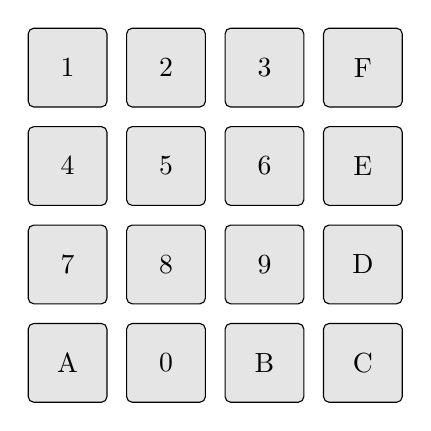
\begin{tikzpicture}
	\def\xAbstand{1.25cm}
	\def\yAbstand{\xAbstand}
	\node[rectangle,rounded corners=2pt,draw, minimum size=1cm,fill=black!10] (d) at (\xAbstand*0,\yAbstand*0) {A};
	\node[rectangle,rounded corners=2pt,draw, minimum size=1cm,fill=black!10] (d) at (\xAbstand*1,\yAbstand*0) {0};
	\node[rectangle,rounded corners=2pt,draw, minimum size=1cm,fill=black!10] (d) at (\xAbstand*2,\yAbstand*0) {B};
	\node[rectangle,rounded corners=2pt,draw, minimum size=1cm,fill=black!10] (d) at (\xAbstand*3,\yAbstand*0) {C};
	%
	\node[rectangle,rounded corners=2pt,draw, minimum size=1cm,fill=black!10] (d) at (\xAbstand*0,\yAbstand*1) {7};
	\node[rectangle,rounded corners=2pt,draw, minimum size=1cm,fill=black!10] (d) at (\xAbstand*1,\yAbstand*1) {8};
	\node[rectangle,rounded corners=2pt,draw, minimum size=1cm,fill=black!10] (d) at (\xAbstand*2,\yAbstand*1) {9};
	\node[rectangle,rounded corners=2pt,draw, minimum size=1cm,fill=black!10] (d) at (\xAbstand*3,\yAbstand*1) {D};
	%
	\node[rectangle,rounded corners=2pt,draw, minimum size=1cm,fill=black!10] (d) at (\xAbstand*0,\yAbstand*2) {4};
	\node[rectangle,rounded corners=2pt,draw, minimum size=1cm,fill=black!10] (d) at (\xAbstand*1,\yAbstand*2) {5};
	\node[rectangle,rounded corners=2pt,draw, minimum size=1cm,fill=black!10] (d) at (\xAbstand*2,\yAbstand*2) {6};
	\node[rectangle,rounded corners=2pt,draw, minimum size=1cm,fill=black!10] (d) at (\xAbstand*3,\yAbstand*2) {E};
	%
	\node[rectangle,rounded corners=2pt,draw, minimum size=1cm,fill=black!10] (d) at (\xAbstand*0,\yAbstand*3) {1};
	\node[rectangle,rounded corners=2pt,draw, minimum size=1cm,fill=black!10] (d) at (\xAbstand*1,\yAbstand*3) {2};
	\node[rectangle,rounded corners=2pt,draw, minimum size=1cm,fill=black!10] (d) at (\xAbstand*2,\yAbstand*3) {3};
	\node[rectangle,rounded corners=2pt,draw, minimum size=1cm,fill=black!10] (d) at (\xAbstand*3,\yAbstand*3) {F};
	%
	\end{tikzpicture}
	\unterschrift{Tastenfeld}{eigene Ausarbeitung}{}
	\label{fig: tastenfeld}
\end{figure}
%
\begin{table}[h]
	\centering
	\begin{tabular}{ c l } 
		\toprule
		\textbf{Keyboard-Taste} & \textbf{Funktion} \\\toprule
		0 & nicht belegt\\\hline
		1 & nicht belegt\\\hline
		2 & erhöhe max. Geschwindigkeit um \stepSizeMotor\\\hline
		3 & nicht belegt\\\hline
		4 & Start Profil links\\\hline
		5 & Start Profil rechts\\\hline
		6 & nicht belegt\\\hline
		7 & nicht belegt\\\hline
		8 & verringere max. Geschwindigkeit um \stepSizeMotor\\\hline
		9 & nicht belegt\\\hline
		A & nicht beleg\\\hline
		B & nicht belegt\\\hline
		C & Stopp\\\hline
		D & nicht belegt\\\hline
		E & Auswahl \modeB \\\hline
		F & Auswahl \modeA \\\hline
	\end{tabular}
	\unterschrift{Funktionen des Tastenfeldes}{eigene Ausarbeitung}{}
	\label{fig: funktionen tastenfeld}
\end{table}
%
\chapter{Kommunikation zwischen den Förderbändern und Master}
%
\begin{table}[h]
	\centering
	\noindent\adjustbox{max width=\textwidth}{%falls größer als \textwidth, wird das Bild verkleinert
	\begin{threeparttable}
	\begin{tabular}{cp{3.25cm}p{6cm}} 
		\toprule
		\textbf{Befehl} & \textbf{Device} & \textbf{Funktion} \\\toprule
		\enquote{Request\delimiterKom}	& linkes Förderband, Master	& Anfrage für die Übergabe des Paketes.\\\hline
		\enquote{Ready\delimiterKom}	& rechtes Förderband, eigenes	& Antwort auf die \request Anfrage, wenn kein Paket vorhanden ist.\\\hline
		\enquote{Release\delimiterKom}	& rechtes Förderband, eigenes	& Rückmeldung, dass das Paket erfolgreich übernommen wurde.\\\hline
		\enquote{Wait\delimiterKom}	& rechtes Förderband, eigenes	& Antwort auf die \request Anfrage, wenn das Paket vorhanden ist.\\\hline
		\enquote{Right 91.0.0.k\delimiterKom}\tnote{a}	& Master	& \glsentryshort{ip}-Adresse des rechten Förderbandes \\\hline
	\end{tabular}
	\unterschrift{Kommunikation zwischen den Förderbändern und Master}{eigene Ausarbeitung}{}
	\label{tab: kommunikation forderbander master}
	\begin{tablenotes}
		\footnotesize
		\item [a] k steht für eine ganze Zahl von 1-90 und 92-254.
	\end{tablenotes}
\end{threeparttable}
}
\end{table}
%
\chapter{\glsentryshort{telnet} Kommunikation}
%
\begin{table}[h]
	\centering
	\begin{tabular}{ c l } 
		\toprule
		\textbf{Befehl} & \textbf{Funktion} \\\toprule
		stop & Abbruch des Geschwindigkeitsprofils \pfeil Stoppen des Motors\\\hline
		local & Auswahl Local Mode\\\hline
		chain & Auswahl Chain Mode\\\hline
		left & Start Profil links\\\hline
		right & Start Profil rechts\\\hline
		plus & erhöhe max. Geschwindigkeit um \stepSizeMotor\\\hline
		minus & verringere max. Geschwindigkeit um \stepSizeMotor\\\hline
	\end{tabular}
	\unterschrift{\glsentryshort{telnet} Kommunikation}{eigene Ausarbeitung}{}
	\label{tab: telnet kommunikation}
\end{table}
%
\chapter{Kalman Filter}\label{sec:kalmann implementation}
%
Nach folgenden Gleichungen ist der Kalman Filter implementiert\footnote{Hier kann der Code heruntergeladen werden: \url{https://github.com/bachagas/Kalman}.\\
In \url{http://interactive-matter.eu/blog/2009/12/18/filtering-sensor-data-with-a-kalman-filter/} ist der 1D Kalman Filter beschrieben.}.
%
\begin{align}
p &= p +q\\
k &= \frac{p}{p+r}\\
x &= k \cdot \left(\text{Messwert} - x\right)\\
p &= \left(1-k\right)\cdot p\\
p&\ldots \text{erwarteter Fehler}\\
r &\ldots \text{Sensorrauschen}\\
q &\ldots \text{Prozessrauschen}\\
k &\ldots \text{Kalman Verstärkung}\\
x &\ldots \text{gefilterter Wert}
\end{align}
%
\chapter{Code der Statemachine}\label{sec: code statemachin}
%
%\section{Statemachine}
%
\lstinputlisting[language=C++,caption=Statemachine mit den Membermethoden]{./img/listings/systemManager.cpp}
%
\end{document}